\documentclass{article}
\usepackage[utf8]{inputenc}
\usepackage[margin = 0.8in]{geometry}
\usepackage{graphicx}
\usepackage{amsmath, amssymb}
\usepackage{subcaption}
\usepackage{multirow}
\usepackage{float}


\title{RBE502 - Homework Set 1}
\author{Keith Chester}
\date{Due date: September 7, 2021}

\begin{document}
\maketitle

\section*{Problem 1}

In this problem we are given a system of a mass at the end of a pendulum. We are given that the differential equation of motion for the system is \[ml^2\dot y=mglsin(q)+u\]
If we choose a control function such that...
\[u=-mglsin(q)-k_1q-k_2\dot q\]
...for \(k_1,k_2>0\), we can solve for the controller by plugging in the \(u\) value.

\[ml^2\ddot q =mglsin(q)-mglsin(q)-k_1q+k_2\dot q\]
\[ml^2\ddot q + k_2\dot q + k_1 q = 0\]

...which has the characteristic function

\[ml^2\lambda + k_2\lambda + k_1\]
...with roots solved via the quadratic formula:
\[ \frac{-k_2^2 \pm \sqrt{k_2^2-4ml^2k_1}}{2ml^2}\]

This ultimately gives us the equation of

\[q = c_1e^{\frac{-k_2^2 + \sqrt{k_2^2-4ml^2k_1}}{2ml^2}} + c_2e^{\frac{-k_2^2 - \sqrt{k_2^2-4ml^2k_1}}{2ml^2}}\]

\[\lim_{t \to \infty} q(t) = 0 = c_1e^{-\infty}+c_2e^{-\infty}\]
\[c_1+c_2 = 0\]

This controller is a PD controller (proportional and derivative). The proportional aspect of the controller will rapidly correct for errors, causing the control system to move the pendulum quickly to the desired portion.

The derivative portion of the controller will attempt to adjust for overshoot from the controller by adjusting according to the rate of change of the error over time. This slows down the proportional response as it approaches the goal.

This produces a fast reacting control system that \textbf{can} reach an equilibrium at the desired point, but may, due to the tuning of the constants, fail to do so. This is because it lacks an integral control component. This component would adjust for small errors over time. This means that a controller tuned incorrectly would still reach the correct value over a long enough period of time and not oscillate. This also means that small deviations from the desired process, IE small errors, would eventually adjust and be fixed. Without the integral portion, small errors may be a long time in being adjusted for if at all.


\section*{Problem 2}

In this problem we look at a system of a 1 dimensional minecart on a frictionless path. Here, the equation for the system is represented as

\[m\dot v = u +\phi(t)\]

where \(u\) is our control system, set to:

\[u=k_p(s-v)+k_d(0-\dot v)=k_ps-k_pv-k_d\dot v\]

which plugged into our systems equation:

\[(m+k_d)\dot v + k_p v = k_p s + \phi(t)\]

We will attempt to find the upperbound for \(\mid v \mid\) as \(t \to \infty\) . To do this, first we shall rewrite our equation in a form of \(\frac{dy}{dt}+ay=g(t)\).

\[\dot v + \frac{k_p v}{m+k_d}= \frac{k_p s + \phi(t)}{m+k_d}\]

By working our system equation into this form, we can now utilize a common form for solving differential equations via an integrating factor. Specifically, that $\frac{dy}{dt+ay=g(t)}$ leads to a $\mu (t)=e^{\int a dt}$, and a solution in the form of $ y = \frac{1}{\mu(t)} \int \mu(s)g(s) ds + c $. Applying this, we have a $\mu(t)$ of:

\[\mu(t) = e^{\frac{k_p}{m+k_d}t}\]

...and a solution of:

\[v = e^{-\frac{k_p}{m+kd}t} \int {e^{\frac{k_p}{m+k_d}t}(\frac{k_p s + \phi(t)}{m + k_d})} \,dt + c_1 e^{-\frac{k_p}{m+kd}t} \]

...and if we expand our integral into two separate integrals: 

\[v = e^{-\frac{k_p}{m+kd}t} \int \frac{e^{\frac{k_p}{m+k_d}t} s k_p}{m+k_d} dt + e^{-\frac{k_p}{m+kd}t} \int \frac{e^{\frac{k_p}{m+k_d}t} \phi(t)}{m + k_d} \,dt + c_1 e^{-\frac{k_p}{m+kd}t}\]

...where we can easily take care of one of the integrals:

\[v = e^{-\frac{k_p}{m+kd}t} e^{\frac{k_p}{m+k_d} t } s + e^{-\frac{k_p}{m+kd}t} \int \frac{e^{\frac{k_p}{m+k_d}t} \phi(t)}{m + k_d} \,dt + c_1 e^{-\frac{k_p}{m+kd}t}\]

...which simplifies down to:

\[v = s + e^{-\frac{k_p}{m+kd}t} \int \frac{e^{\frac{k_p}{m+k_d}t} \phi(t)}{m + k_d} \,dt + c_1 e^{-\frac{k_p}{m+kd}t}\]

From here, we can utilize integration by parts for our remaining integral. For our purposes:

\[\int u v \,dt = u \int v \,dt - \int (\dot u \int v \,dt)\,dt\]

...where \(u = \frac{\phi(t)}{m+k_d}\), \(\dot u = \frac{\dot \phi(t)}{m+k_d}, v = e^{\frac{k_p}{m+k_d}t}\), and \(\int v = \frac{e^{\frac{k_p}{m+k_d}t}(m+k_d)}{k_p}\), thus making our second integral:

\[\frac{\phi(t)}{m+k_d} \frac{e^{\frac{k_p}{m+k_d}t}(m+k_d)}{k_p} - \int { \frac{\dot \phi(t)}{m+k_d} \frac{e^{\frac{k_p}{m+k_d}t}(m+k_d)}{k_p}}\]

which simplifies to

\[ \frac{\phi(t) e^{\frac{k_p}{m+k_d}t}}{kp} - \int \frac{\dot \phi(t) e^{\frac{k_p}{m+k_d}t}}{k_p} \]

When we plug this back into our prior equation:

\[v = s + e^{-\frac{k_p}{m+kd}t} (\frac{\phi(t) e^{\frac{k_p}{m+k_d}t}}{kp} - \int \frac{\dot \phi(t) e^{\frac{k_p}{m+k_d}t}}{k_p}) + c_1 e^{-\frac{k_p}{m+kd}t}\]

which simplifies further to:

\[v = s + \frac{\phi(t)}{kp} - e^{-\frac{k_p}{m+kd}t} \int \frac{\dot \phi(t) e^{\frac{k_p}{m+k_d}t}}{k_p} + c_1 e^{-\frac{k_p}{m+kd}t}\]


We take the limit of our resulting system equation as \(t \to \infty\):

\[\lim_{t \to \infty} v(t) = s + \frac{\phi(t)}{k_p} - e^{-\infty} \int \frac{e^{\infty} \dot \phi(t)}{m+k_d} \,dt + c_1 e^{-\infty}\]

...and since \(e^{-\infty} = 0\):

\[\lim_{t \to \infty} v(t) = s + \frac{\phi(t)}{k_p}\]

Since \(\phi(t) < a\) as per our description, we can thus say that the upperbound velocity of the given problem is defined by

\[v(t) < s + \frac{a}{k_p}\]

\section*{Problem 3}

\subsection*{Part 1}

Figure~\ref{fig:part-1_result} illustrates the response of the system for $\phi(e) = e$ and $r = 1$ for the parameters listed in Table~\ref{tab:paramters}.
\begin{table}[H]
    \centering
    \begin{tabular}{|r|l|}
        \hline
        Simulation time & $t_0 = 0$, $t_f = 10$  \\
        \hline
        Initial conditions & $y(t_0) = \dot{y}(t_0) = 0$\\
        \hline
        System parameters & $m = 1$, $b = 2$, and $k = 4$\\
        \hline
        Reference Input & $r = 1$\\
        \hline
    \end{tabular}
    \caption{System parameters used in the simulation}
    \label{tab:paramters}
\end{table}
Based on the simulation results, we have $e(10) \approx 1 - 0.83 \approx 0.17 $ . Much like the first question on the week 1 quiz, the error does not approach reach zero and will not stand in the correct desired position, $r$.
\begin{figure}[H]
    \centering
    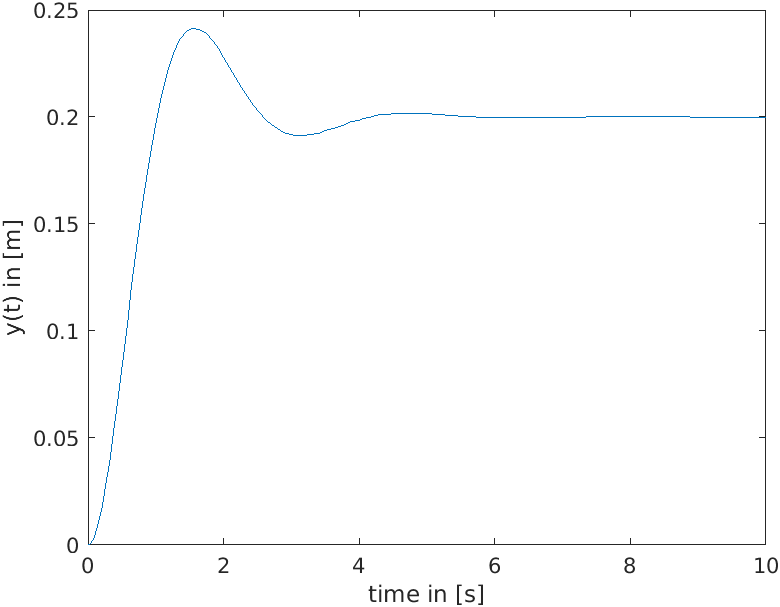
\includegraphics[width = 0.4\textwidth]{figures/figure_1.png}
    \caption{System response for $\phi(e) = e$ and $r = 1$.}
    \label{fig:part-1_result}
\end{figure}


\subsection*{Part 2}
Figure~\ref{fig:part-2_results} illustrates the response of the system to PID controller
\begin{equation}
    \label{eq:pid}
    u(t) = k_p e(t) + k_i \int_{t_0}^t e(\tau)\,d\tau + k_d\dot{e}(t), 
\end{equation}
for the 3 case studies as listed in Table~\ref{tab:part-2}. Here, $k_p$ causes large jumps towards the desired position, sometimes resulting in overshooting the desired position entirely. $k_i$, adjusts the system's response until it reaches 0 over time. The swings that the $k_i$ parameter applies to the can be large enough to still contribute to overshoots when trying to adjust. The $k_d$ parameter controls the derivative term of the control system, reacting to the response of the system and "smoothing it out" to prevent overshooting. It does not significantly contribute to the actual error correction itself, however.
%
\begin{table}[H]
    \centering
    \begin{tabular}{|c|c|c|c||c|c|c|}
        \hline
         Case Study & $k_p$ & $k_i$ & $k_d$ & $e(t_f)$ & $u(t_f)$ & $J$  \\
        \hline\hline
        \multirow{3}{*}{I} &  5 & 0 & 0 & 0.4444 & 2.2221 & 4.5682\\
                           & 10 & 0 & 0 & 0.2857 & 2.8570 & 2.9622\\
                           & 20 & 0 & 0 & 0.1666 & 3.3327 & 1.9038\\
        \hline
        \multirow{3}{*}{II} & 10 &  2 & 0 & 0.0299 & 3.888 & 1.0425\\
                            & 10 &  5 & 0 & -0.0032 & 4.0077 & 0.9744\\
                            & 10 & 10 & 0 & -0.0021 & 3.9757 & 1.6368\\
        \hline
        \multirow{3}{*}{III} & 10 & 0 &  2 & 0.2857 & 2.5871 & 3.0615\\
                             & 10 & 0 &  5 & 0.2857 & 2.8571 & 3.2145\\
                             & 10 & 0 & 10 & 0.2857 & 2.8571 & 3.4696\\
        \hline
    \end{tabular}
    \caption{Results of the three case studies for Part 2.}
    \label{tab:part-2}
\end{table}
%
The performance index $J \in \mathbb{R}^+$ defined as
\begin{equation}
    J = \int_{t_0}^{t_f} |e(t)|\,dt = \int_{t_0}^{t_f} |r(t) - y(t)|\,dt,
\end{equation}
The performance index $J$ is a measure of a control system based on how quickly the system converges to a low or zero error. The lower the score the smaller the total error is at a faster rate. Thus control systems that converge faster or closer to the desired position will have a lower J score.

\begin{figure}[H]
    \centering
    \begin{subfigure}{0.325\textwidth}
        \centering
        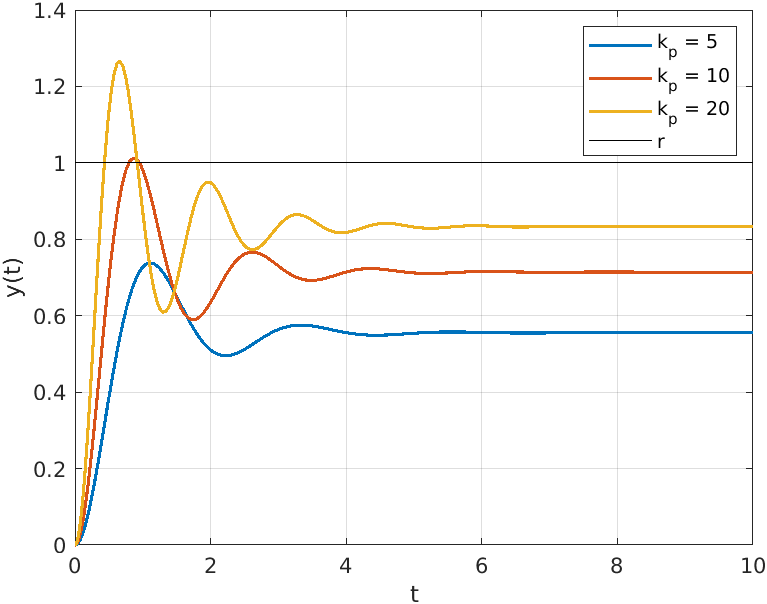
\includegraphics[width = \textwidth]{figures/part_2_kp.png}
        \caption{Case study I}
    \end{subfigure}
    \begin{subfigure}{0.325\textwidth}
        \centering
        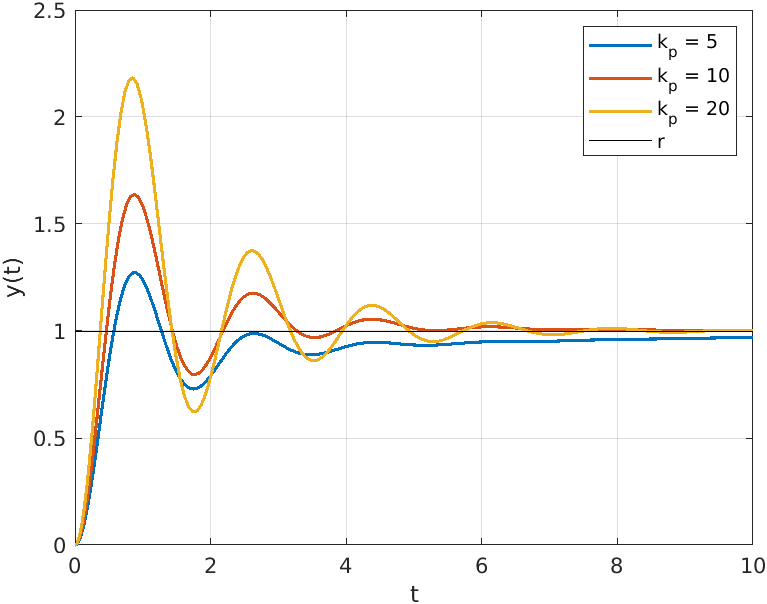
\includegraphics[width = \textwidth]{figures/part_2_ki.png}
        \caption{Case study II}
    \end{subfigure}
    \begin{subfigure}{0.325\textwidth}
        \centering
        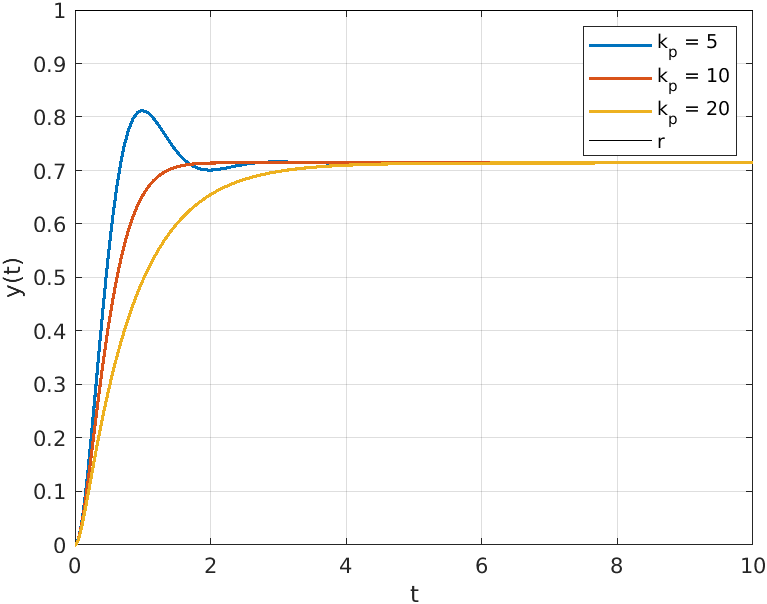
\includegraphics[width = \textwidth]{figures/part_2_kd.png}
        \caption{Case study III}
    \end{subfigure}
    \caption{System response to PID controller for the three case studies of Part 2.}
    \label{fig:part-2_results}
\end{figure}

Similar to the second question on the week 1 quiz, the case 2 study provides both a proportional and integral portion of a control equation. This results in better performance, getting the error closer to zero over time.

\subsection*{Part 3}

Figure~\ref{fig:part-3_results} illustrates the response of the system to PID controller (\ref{eq:pid}) when $r(t) = \cos(t)$. The performance measure $J$ for all case studies is tabulated in Table~\ref{tab:part-3}


\begin{table}[H]
    \centering
    \begin{tabular}{|c|c|c|c||c|c|}
        \hline
         Case Study & $k_p$ & $k_i$ & $k_d$ & $J$  \\
        \hline\hline
        \multirow{3}{*}{I} &  5 & 0 & 0  & 4.2709 \\
                           & 10 & 0 & 0  & 2.7392\\
                           & 20 & 0 & 0  & 1.6144\\
        \hline
        \multirow{3}{*}{II} & 10 &  2 & 0 & 2.9135 \\
                            & 10 &  5 & 0 & 3.2039 \\
                            & 10 & 10 & 0 & 3.7227 \\
        \hline
        \multirow{3}{*}{III} & 10 & 0 &  2 & 2.2632 \\
                             & 10 & 0 &  5 & 1.7439 \\
                             & 10 & 0 & 10 & 1.4065 \\
        \hline
    \end{tabular}
    \caption{Results of the three case studies for Part 3.}
    \label{tab:part-3}
\end{table}
    
\begin{figure}[H]
    \centering
    \begin{subfigure}{0.325\textwidth}
        \centering
        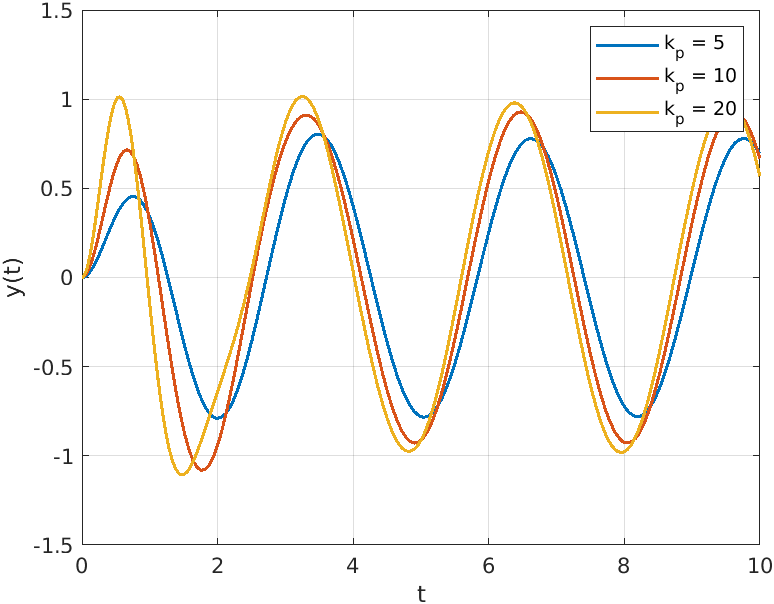
\includegraphics[width = \textwidth]{figures/part_3_kp.png}
        \caption{Case study I}
    \end{subfigure}
    \begin{subfigure}{0.325\textwidth}
        \centering
        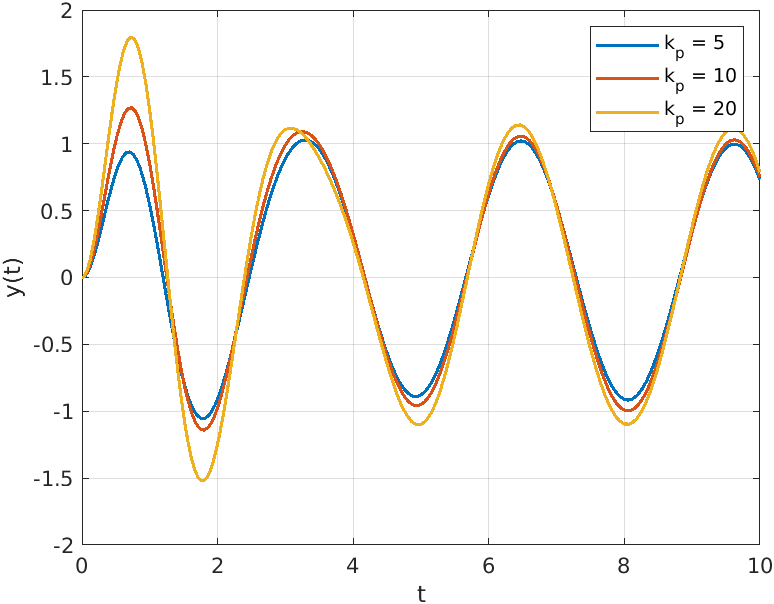
\includegraphics[width = \textwidth]{figures/part_3_ki.png}
        \caption{Case study II}
    \end{subfigure}
    \begin{subfigure}{0.325\textwidth}
        \centering
        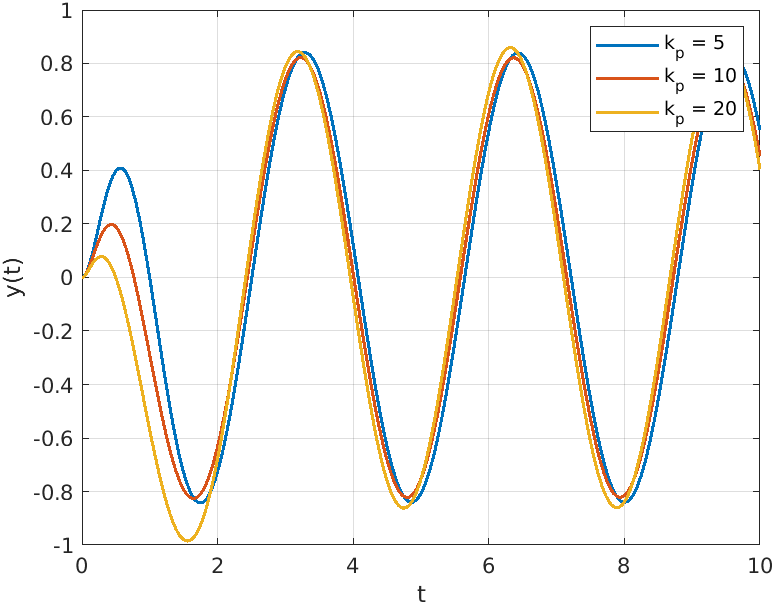
\includegraphics[width = \textwidth]{figures/part_3_kd.png}
        \caption{Case study III}
    \end{subfigure}
    \caption{System response to PID controller for the three case studies of Part 3.}
    \label{fig:part-3_results}
\end{figure}

\end{document}
